\chapter{Progettazione di \textit{NextPyter}}
Il lavoro descritto in questa tesi è il frutto di una seconda iterazione di sviluppo e cambiamenti su codice già esistente. Infatti, è stata ereditata una \textit{codebase}, che verrà indicata con il nome \textit{NextPyter "1.0"}, sulla quale era necessario effettuare modifiche per migliorare il progetto esistente, oltre che migrare la piattaforma ad una soluzione facilmente distribuibile su \textit{Kubernetes}. \newline
Verrà esplorato brevemente l'ottimo lavoro effettuato in precedenza e la sua architettura, verrà fatta un'analisi del sistema a quello stato e, successivamente, verrà descritto il passaggio da \textit{NextPyter "1.0"} a \textit{NextPyter "2.0"}, che rappresenta lo stato del progetto alla stesura di questa tesi. 
\section{Obiettivi di \textit{NextPyter}}
In generale, \textit{NextPyter} vuole essere una piattaforma tramite la quale sia possibile condividere in maniera efficiente dati e codice a scopo di ricerca. Come si può intuire dal nome, per realizzare gli obiettivi posti, \textit{NextPyter} fa uso di \textit{Nextcloud}, per la gestione dei file, e di \textit{JupyterLab}, che accederà ai file gestiti da Nextcloud.

\subsection{Containerizzazione}
Il fondamento cardine di \textit{NextPyter}, per entrambe le versioni, è la \textit{containerizzazione}, ovvero la pratica di distribuire software mediante l'utilizzo di \textit{container}\footnote{https://en.wikipedia.org/wiki/Docker\_(software)}, generalmente Docker, ambienti di esecuzione completamente isolati rispetto al resto del sistema. 
\newline
Per creare ambienti di sviluppo (i Jupyter Notebook) quanto più sicuri possibile, l'utilizzo di tecnologie di \textit{containerizzazione} è fondamentale, per la semplicità d'uso e la modularità che questo approccio offre.\newline
Tramite cosiddette \textit{immagini}\footnote{https://www.techtarget.com/searchitoperations/definition/Docker-image}, infatti, è possibile eseguire software che richiede numerose dipendenze, come \textit{JupyterLab} e lo stesso \textit{Nextcloud}, in maniera estremamente semplice, utilizzando una sorta di "pacchetto", l'immagine, per l'appunto, che viene scaricato da un registro immutabile\footnote{https://hub.docker.com}. Replicare un ambiente composto da tanti componenti complessi, quindi, è estremamente semplice, se si fa leva su tecnologie di \textit{containerizzazione}, per i vantaggi di distribuzione che questa metodologia offre.

\subsection{Interfaccia grafica familiare}
Per favorire l'utilizzo di \textit{NextPyter}, l'interfaccia deve essere quanto più semplice possibile, per ragione già specificate nell'introduzione di questa tesi. 
\newline
Per questo motivo, come già anticipato, viene usato Nextcloud come interfaccia principale, anche per via del fatto che si tratta di un'affermata soluzione \textit{self-hosted}, con una community sempre più in via di espansione \cite{nextcloud-growing}.

\subsection{Collaborazione in sicurezza}
Accoppiando tecnologie di \textit{containerizzazione} e moderni sistemi di autenticazione si vuole creare un'esperienza utente quanto più sicura possibile. \newline
Oltre alle \textit{policy} di sicurezza sulla gestione dei file che \textit{Nextcloud} già offre, l'obiettivo finale è quello di accoppiare, a ciascun utente, i permessi per creare, visualizzare e modificare determinati \textit{notebook} in maniera completamente privata, permettendo la selettiva condivisione di questi ultimi.
\newline
L'isolamento, quindi, deve avvenire non solo a livello di permesso sui file, ma anche a livello di \textit{notebook}.

\subsection{FLOSS}
Per favorire lo sviluppo di \textit{NextPyter} è stato deciso di adottare la filosofia FLOSS\footnote{https://www.gnu.org/philosophy/floss-and-foss.en.html}, \textit{Free/Libre And Open Source Software}. Il codice sorgente del progetto è pubblico e consultabile su una \textit{repository GitLab}\footnote{https://gitlab.com/nextpyter/}. Tutti i componenti sono sotto licenza \textit{MIT} e sono liberamente modificabili da chiunque voglia partecipare allo sviluppo di questa piattaforma.

\newpage

\section{NextPyter \textit{"1.0"}}
Per poter parlare dell'evoluzione della piattaforma \textit{NextPyter}, è opportuno introdurre brevemente lo stato di quest'ultima prima che iniziasse il lavoro di revisione che verrà descritto successivamente.
\newline
Per ultieriori dettagli su questa implementazione, è opportuno consultare la tesi del progetto originale \cite{nextpyter-1}.
\newline
\begin{figure}[h]
    \centering
    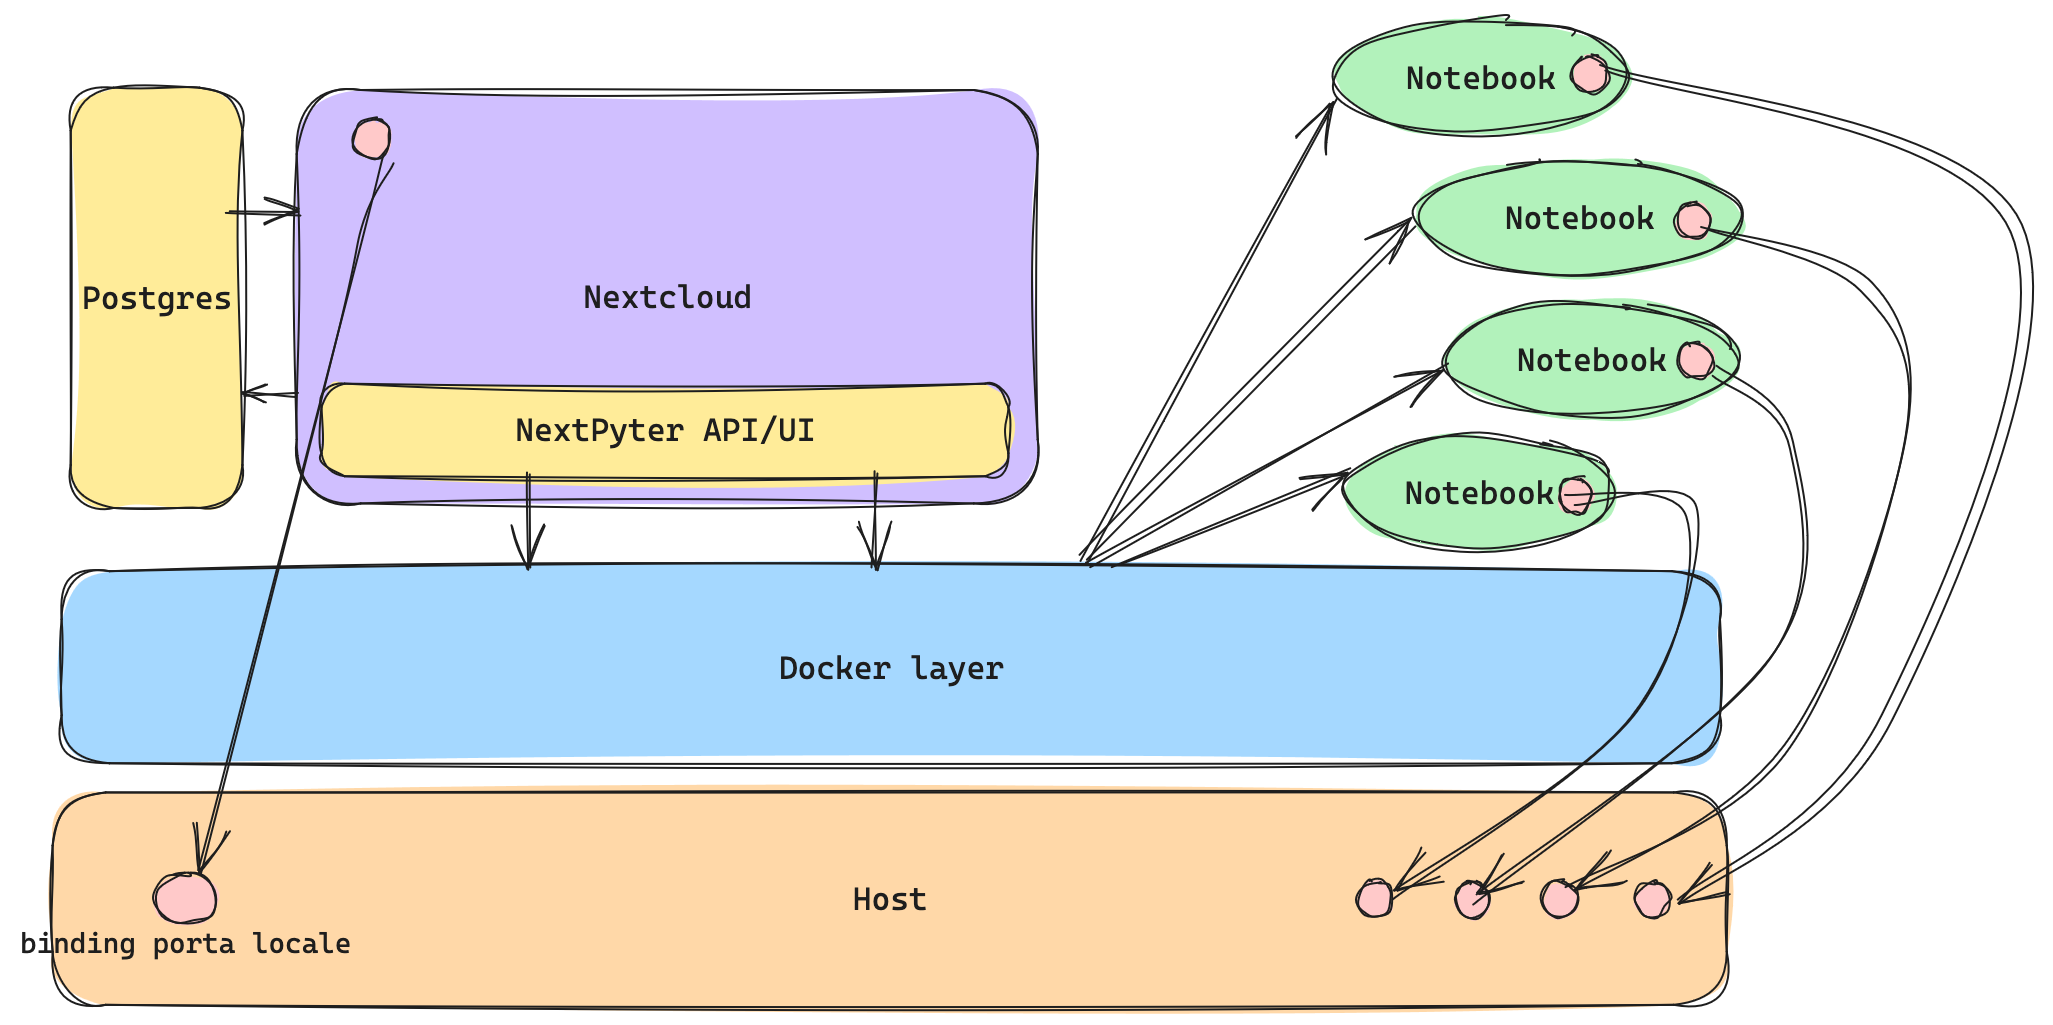
\includegraphics[width=1\textwidth]{files/images/nextpyter-1-0.png}
    \caption{Schema architetturale NextPyter "1.0"}
    \label{fig:nextpyter-1-0-architecture}
\end{figure}
\newline
In figura \ref{fig:nextpyter-1-0-architecture} è possibile vedere uno schema architetturale di alto livello della piattaforma \textit{"1.0"} e i vari componenti che la realizzano:
\begin{itemize}
    \item Un'installazione di Nextcloud e il relativo database (Postgres) che utilizza per gestire utenti, permessi e quant'altro;
    \item Un'applicazione \textbf{installata all'interno di Nextcloud}, ovvero \textit{NextPyter} vero e proprio. Questo applicativo si interfaccerà direttamente con Docker per creare e gestire i \textit{container} relativi ai notebook. Questo componente comprenderà sia un'API per l'interfaccia con Docker, che il componente relativo alla UI e alla visualizzazione dei dati;
    \item Notare che ciascun notebook avrà un \textit{binding} di una porta locale rispetto all'host sul quale Docker sta eseguendo, pertanto \textit{NextPyter} avrà bisogno di trovare una porta libera sull'host prima di creare un container: in questo modo i notebook saranno accessibili dall'esterno.
\end{itemize}
\newpage
\subsection{Funzionamento applicativo \textit{NextPyter} installato su Nextcloud}
L'applicazione installata su Nextcloud regola la creazione, l'avviamento e l'eventuale eliminazione dei notebook Jupyter da Nextcloud.
\newline
In sostanza, è possibile, tramite le estensioni fornite da \textit{NextPyter}, creare delle particolari cartelle che conterranno file relativi a determinati notebook, che verranno eseguiti effettuando determinate chiamate HTTP verso il socket di Docker stesso. 
\newline
Una volta avviato un notebook, sarà possibile accedervi mediante l'utilizzo di un token che viene generato a tempo di esecuzione dall'applicativo stesso, associato all'utente che esegue il notebook, in modo che solo chi ha tale token potrà accedere al container in questione.
\newline
A seguire, alcune immagini che illustrano il funzionamento dell'applicativo.
\newline
\begin{figure}[h]
    \centering
    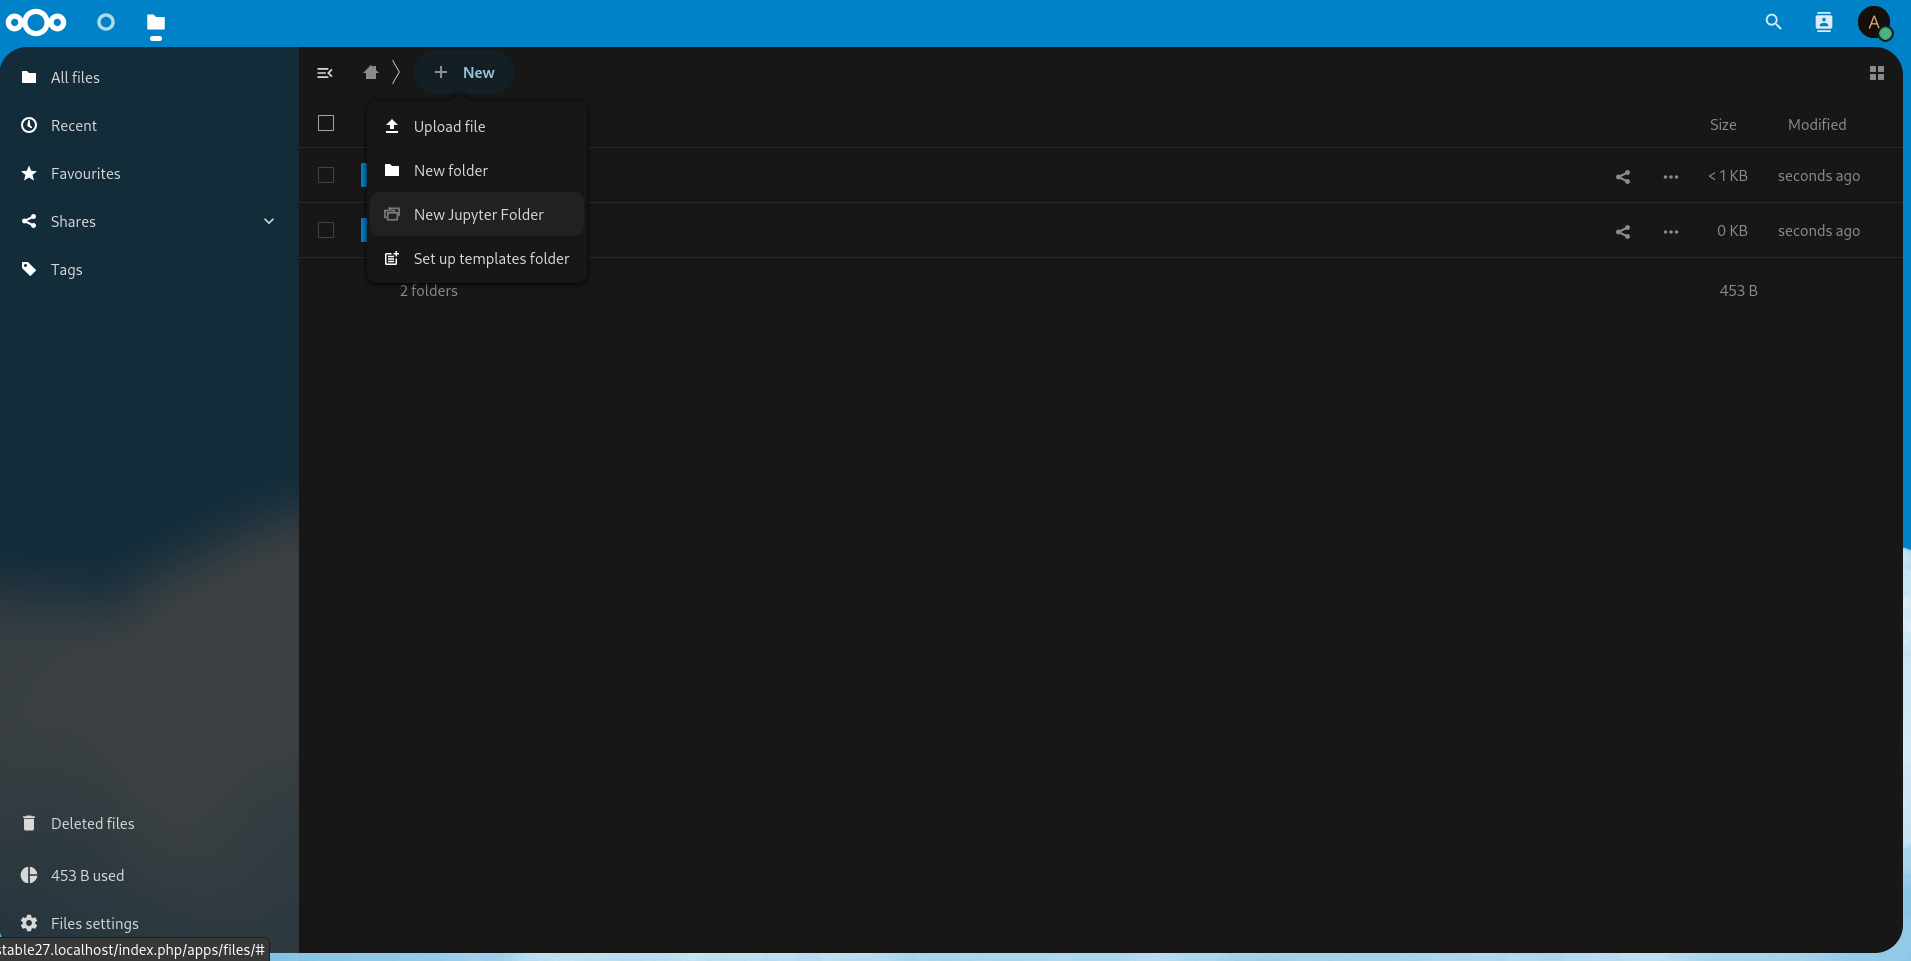
\includegraphics[width=0.75\textwidth]{files/images/example-nextpyter-1-1.png}
    \caption{Interfaccia grafica NextPyter "1.0" - Creazione cartella per notebook Jupyter}
    \label{fig:1.0-example-1}
\end{figure}
\begin{figure}[h]
    \centering
    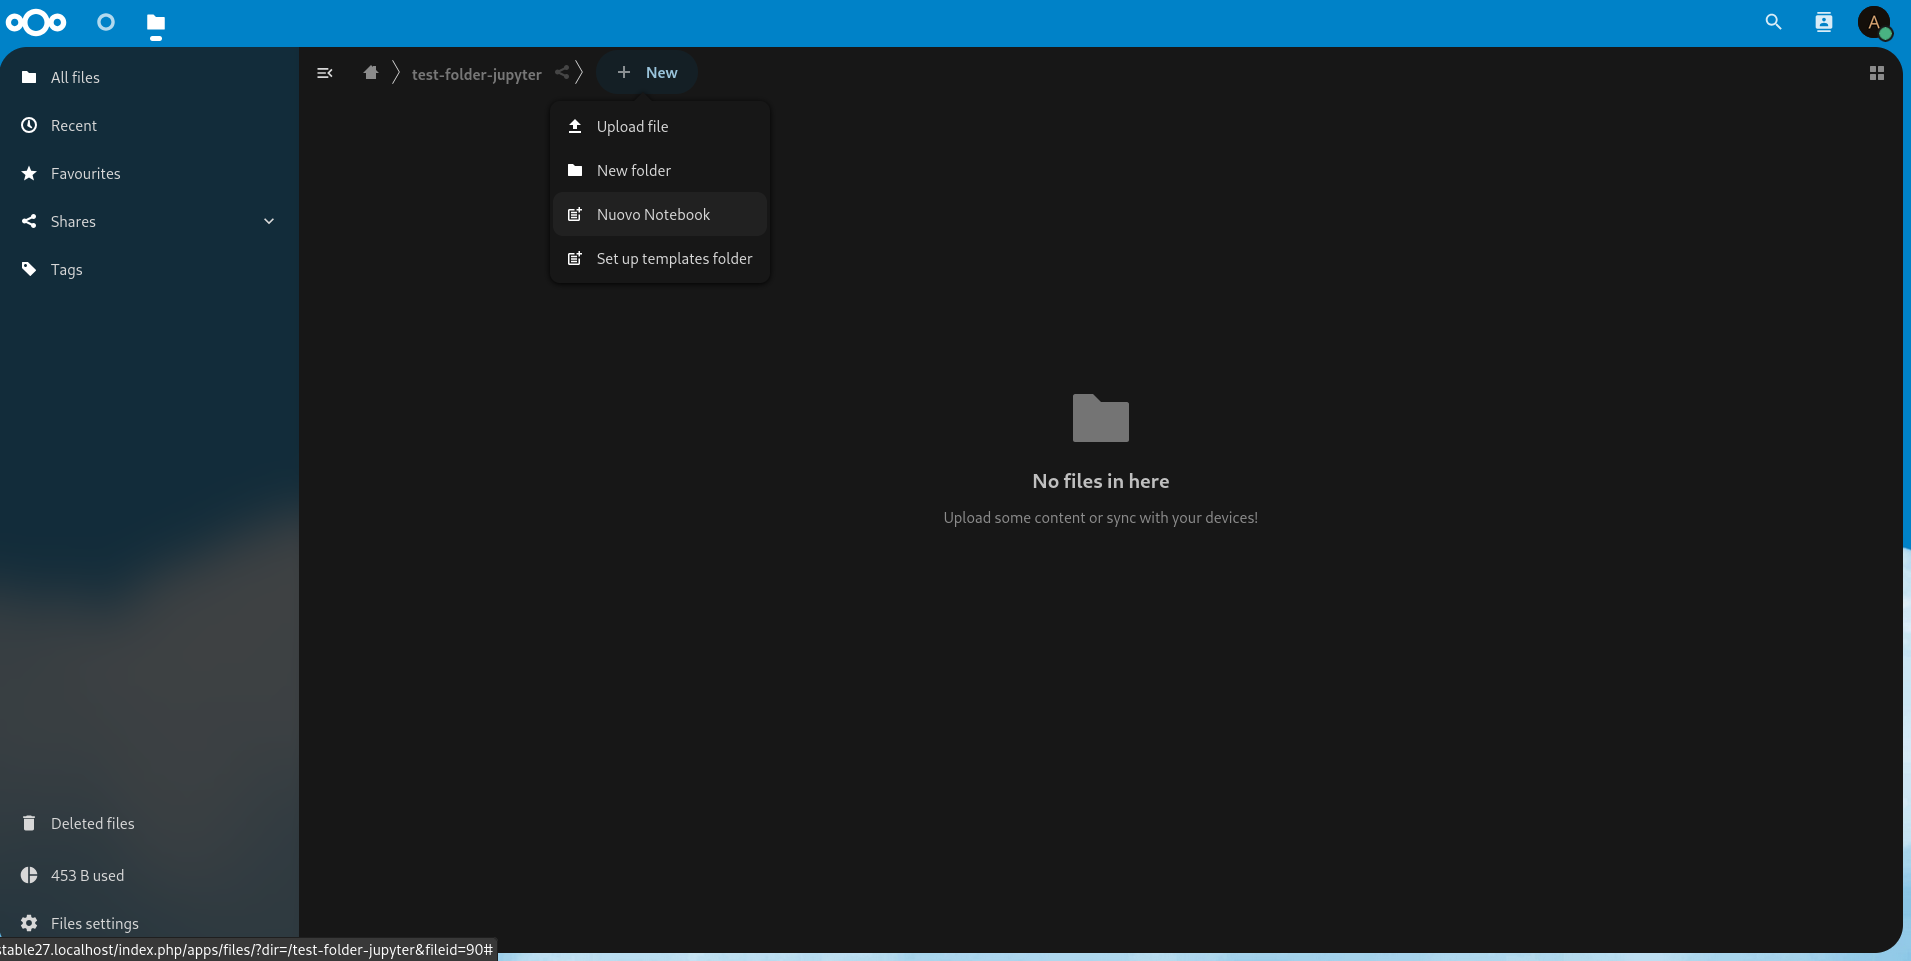
\includegraphics[width=1\textwidth]{files/images/example-nextpyter-1-2.png}
    \caption{Interfaccia grafica NextPyter "1.0" - Creazione notebook dentro la cartella}
    \label{fig:1.0-example-2}
\end{figure}
\begin{figure}[h]
    \centering
    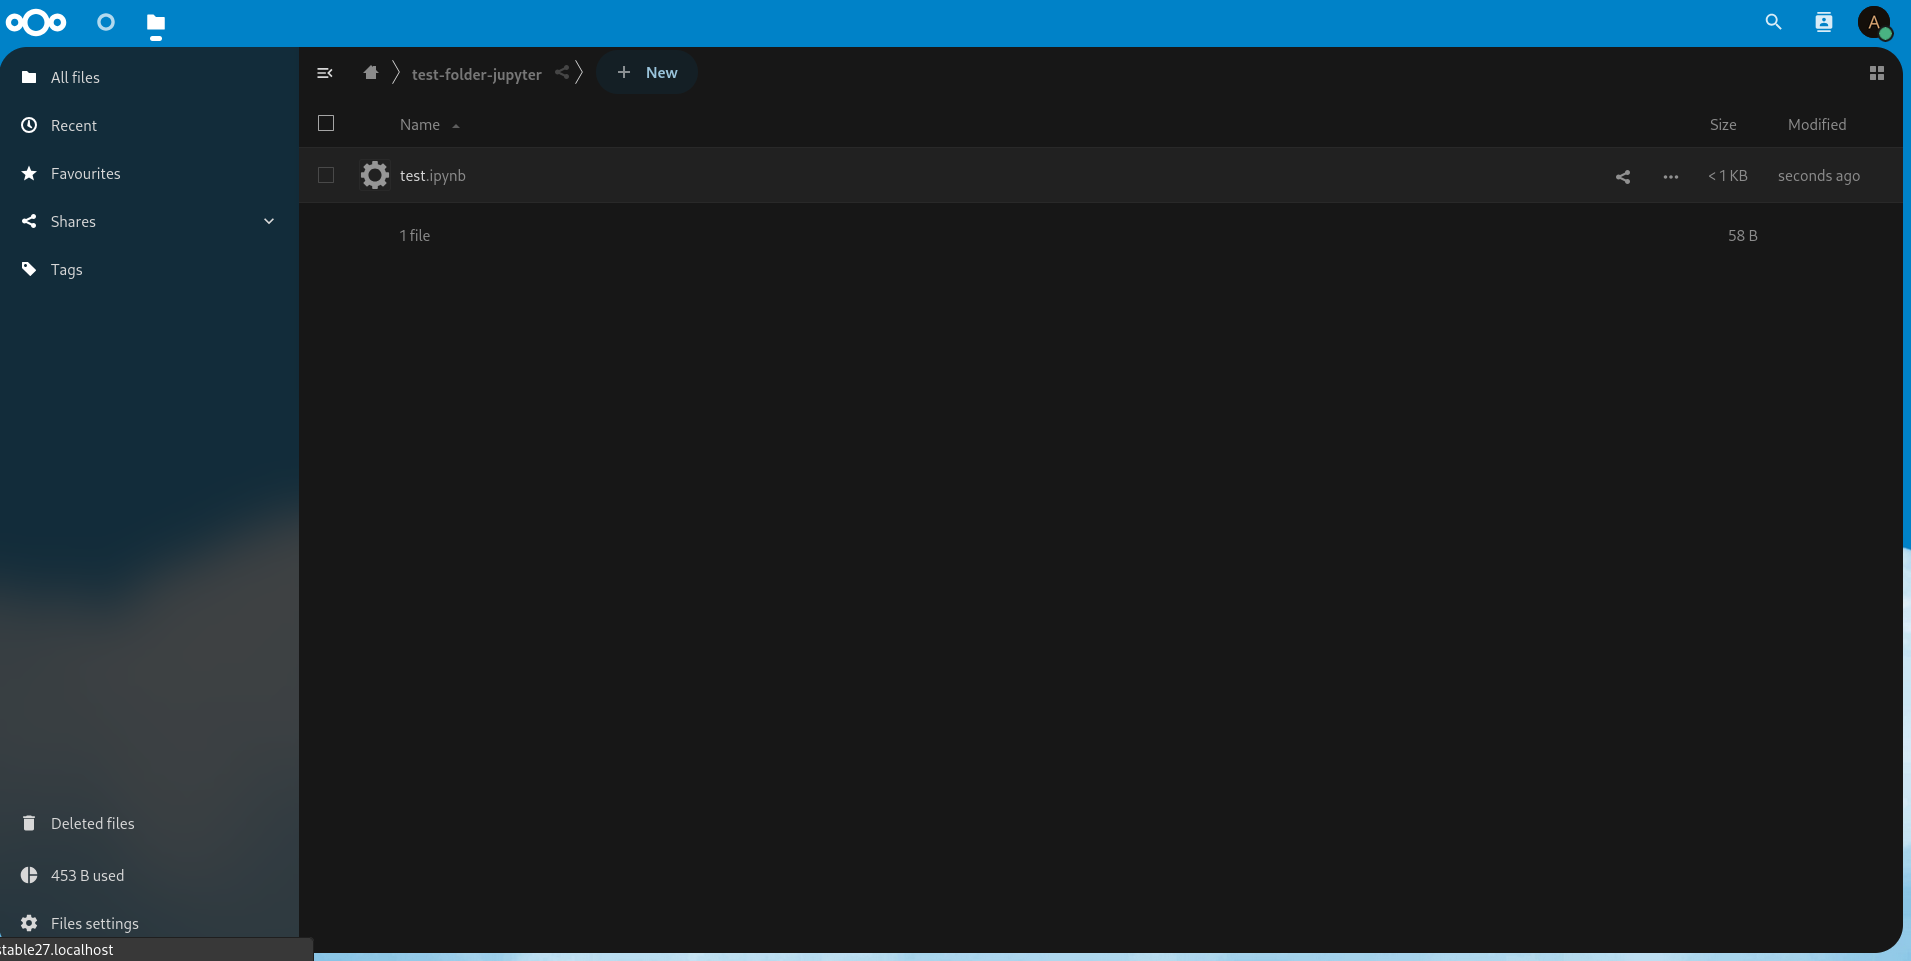
\includegraphics[width=1\textwidth]{files/images/example-nextpyter-1-3.png}
    \caption{Interfaccia grafica NextPyter "1.0" - Notebook creato}
    \label{fig:1.0-example-2}
\end{figure}
\begin{figure}[h]
    \centering
    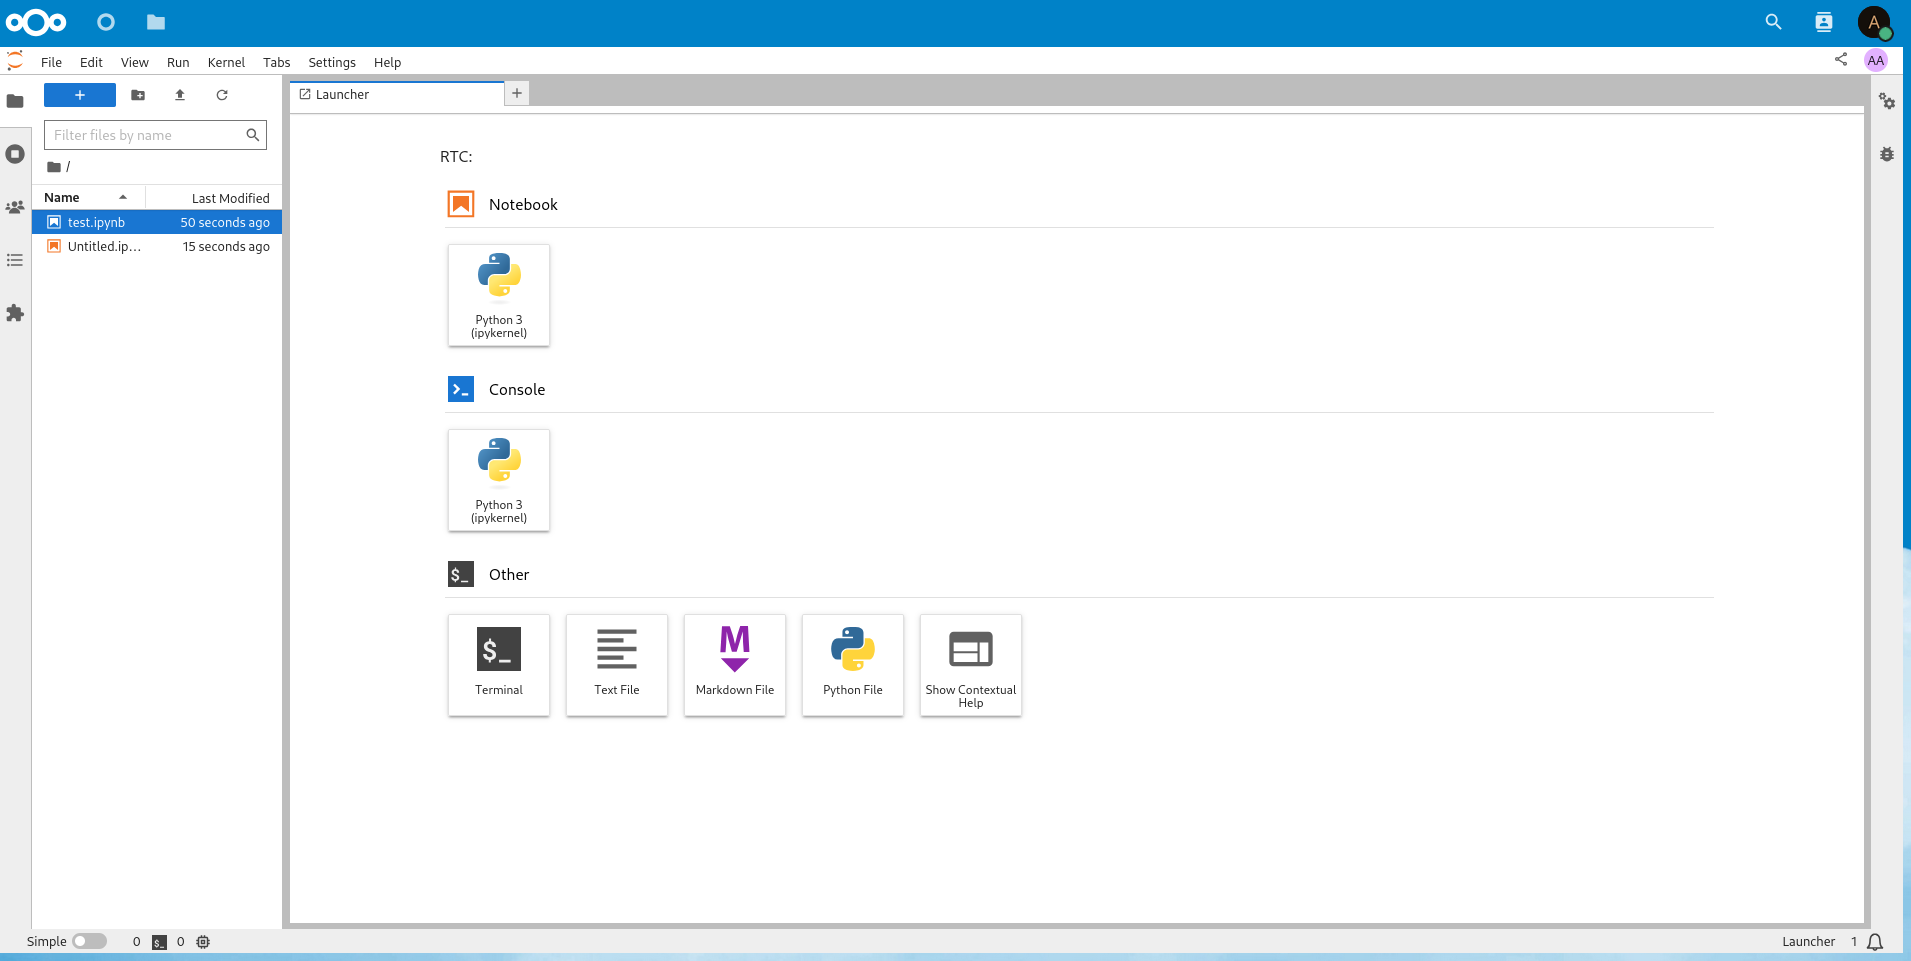
\includegraphics[width=1\textwidth]{files/images/example-nextpyter-1-4.png}
    \caption{Interfaccia grafica NextPyter "1.0" - Avviamento notebook}
    \label{fig:1.0-example-2}
\end{figure}

\subsubsection{Interfacciamento con Docker tramite Docker in Docker (DinD)}
Prima di spiegare effettivamente cosa sia Docker in Docker e come \textit{NextPyter} si interfaccia ad esso, è opportuno capire come Docker esponga le proprie funzionalità a client esterni, tra i quali, fra l'altro, figura il client a linea di comando di Docker stesso.
\newline
Docker è estensibile nel senso che è possibile sfruttare una API HTTP\footnote{https://docs.docker.com/reference/api/engine/}, esposta tramite un socket locale, per poter gestire programmaticamente \textit{container} all'interno dell'host in questione.
\newline
Ad esempio, è possibile interagire in maniera molto semplice con il \textit{daemon} di Docker tramite una semplice chiamata HTTP effettuata, in questo caso, con \textit{cURL}\footnote{https://curl.se/}.
\newline
Supponiamo di eseguire un container con \textit{NGINX} all'interno, usando il comando:
\begin{verbatim}
    docker run --rm -d nginx
\end{verbatim}
A questo punto, è possibile interrogare la REST API di Docker tramite una semplice chiamata \textit{GET} ad un URL specifico:
\begin{verbatim}
    curl --unix-socket /var/run/docker.sock http://localhost/containers/json
    [
    {
        "Id": "61969199e57ac0e1147e6092b110b895c47bc7913734f978377d53c428518107",
        "Names": [
            "/amazing_ride"
        ],
        "Image": "nginx",
        "ImageID": "sha256:8dd77ef2d82eade8...",
        "Command": "/docker-entrypoint.sh nginx -g 'daemon off;'",
        "Created": 1724752281,
        "Ports": [
            {
                "PrivatePort": 80,
                "Type": "tcp"
            }
        ],
        "Labels": {
            "maintainer": "NGINX Docker Maintainers"
        },
        "State": "running",
        "Status": "Up 4 seconds",
        "HostConfig": {
            "NetworkMode": "bridge"
        },
        "NetworkSettings": {
            "Networks": {
                "bridge": {
                    "IPAMConfig": null,
                    "Links": null,
                    "Aliases": null,
                    "MacAddress": "02:42:ac:11:00:02",
                    "NetworkID": "4a20cc24e78576fcd7c04b34a5208...",
                    "EndpointID": "048c2839a30529d26a6635c4af1d43...",
                    "Gateway": "172.17.0.1",
                    "IPAddress": "172.17.0.2",
                    "IPPrefixLen": 16,
                    "IPv6Gateway": "",
                    "GlobalIPv6Address": "",
                    "GlobalIPv6PrefixLen": 0,
                    "DriverOpts": null,
                    "DNSNames": null
                }
            }
        },
        "Mounts": []
    }
]
\end{verbatim}
\newpage
È possibile, ovviamente, eseguire anche un container tramite chiamate HTTP, sempre utilizzando l'API apposita:
\begin{verbatim}
    $ curl --unix-socket /var/run/docker.sock \
        -H "Content-Type: application/json" \
        -d '{"Image": "nginx", "Name": "esempio-nginx"}' \
       -X POST http://localhost/containers/create
    output: {
        "Id": "cf109023d2",
        "Warnings":[]
    }
    $ curl --unix-socket /var/run/docker.sock 
        -X POST http://localhost/v1.46/containers/cf109023d2/start
\end{verbatim}

Ovviamente, usando la chiamata vista in precedenza, si potrà vedere che il container è stato avviato con successo.
\newline
NextPyter fa pesante affidamento, ovviamente, sull'API offerta da Docker, poiché deve programmaticamente gestire il ciclo di vita di container, in base agli eventi che accadono sull'interfaccia utente di Nextcloud. Per fare ciò, la versione \textit{"1.0"} di NextPyter fa uso di due meccanismi principali che abilitano l'interfacciamento con Docker in maniera semplice: un'interfaccia software, DockerClient.php\footnote{https://gitlab.com/frfaenza/NextPyter/-/blob/main/lib/Service/DockerClient.php} e l'utilizzo di una procedura che comunemente viene chiamata \textit{Docker in Docker (DinD)}.
\newline
\textit{DinD} è necessario, poiché, generalmente, l'API HTTP del daemon è disponibile a livello di \textit{host}, quindi solo applicativi che risiedono su di esso (non containerizzati) possono, teoricamente, accedervi. Per aggirare questo limite, è possibile mappare il socket di Docker all'interno dei \textit{container} che ne dovranno fare uso uso, in questo caso quello di \textit{Nextcloud} (al quale accederà l'applicativo NextPyter).
\newline
Utilizzando, ad esempio, Docker Compose è possibile realizzare \textit{DinD} in maniera molto semplice:
\begin{verbatim}
    services:
        ubuntu:
            image: ubuntu
            volumes:
                - /var/run/docker.sock:/var/run/docker.sock:ro
\end{verbatim}
In questo modo si è creato un container basato su \textit{Ubuntu} che ha, montato, il file corrispondente al socket di Docker sull'host: notare come il \textit{mount} venga fatto \textit{read-only}; questo non significa che il socket non sarà scrivibile, ma che il \textit{file} mappato all'interno del container non lo sia. In questo modo si impedisce ad agenti interni al container di \textit{cancellare} il file corrispondente al socket, perché tutti i file \textit{mappati} all'interno di un container, se cancellati, lo saranno anche sull'host.
\newline
A questo punto sarà tranquillamente possibile eseguire i comandi precedentemente visti senza alcun problema, interagendo con Docker \textit{all'interno} di un container.

\newpage

\subsection{Criticità}
A seguito verranno elencate le criticità rilevate nel modello esposto dalla versione \textit{"1.0"}, sostanzialmente il motivo per il quale questa tesi esiste.

\subsubsection{Possibili vulnerabilità dovute a \textit{Docker in Docker}} \label{dind-acceptable}
Sebbene funzionale, l'approccio \textit{Docker in Docker} è generalmente riconosciuto \textit{potenzialmente pericoloso} \cite{dind}, per via del fatto che è possibile, sfruttando eventuali vulnerabilità di applicazioni containerizzate, accedere al socket Docker avendo, di fatto, completo controllo sul \textit{daemon} della macchina host.
\newline
Questa cosa è particolarmente preoccupante se si pensa che \textit{Nextcloud} non è un software che \textbf{nasce} con la pretesa di controllare un ambiente containerizzato, anzi, tutt'altro! Se, per caso, venisse introdotta una vulnerabilità che permette di eseguire codice arbitrario tramite una richiesta HTTP verso un'istanza \textit{Nextcloud} containerizzata, nulla vieterebbe l'attaccante di eseguire una richiesta al socket Docker riproducendo una richiesta simile a quelle viste in precedenza!
\newline
Il problema non è tanto \textit{DinD}, quanto il fatto che il \textbf{software} che ha accesso al socket, in questo caso \textit{Nextcloud}, non sia \textit{adibito specificatamente} alla gestione di questo approccio. 
\newline
In altre parole, \textit{DinD} è accettabile quando, nel container, è presente un software che ha come unico scopo quello di gestire il socket Docker, magari soddisfando richieste derivanti da altri container, in modo da essere l'unico punto di collegamento a Docker nel sistema containerizzato.
\begin{figure}[h]
    \centering
    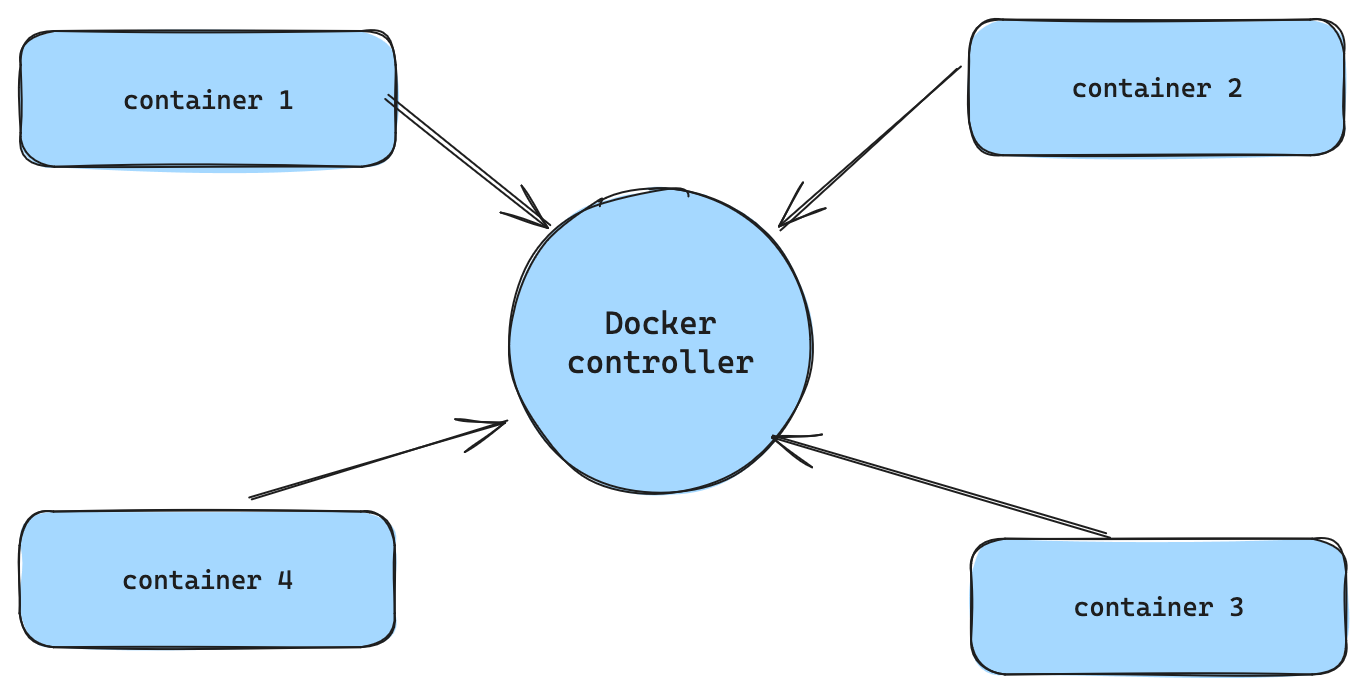
\includegraphics[width=0.75\textwidth]{files/images/dind-solution.png}
    \caption{Schematizzazione architettura accettabile per Docker in Docker}
    \label{fig:dind-acceptable}
\end{figure}
\newline
In figura \ref{fig:dind-acceptable}, infatti, è schematizzata un'architettura \textit{proposta come accettabile} per la gestione di questo approccio. Supponendo, ad esempio, che il \textit{Docker controller} esponga, a sua volta, un'API HTTP che mima quella di Docker (magari limitando l'accesso soltanto a determinati metodi), i container che vogliono consultare l'orchestratore lo potranno fare attraverso il \textit{Docker controller}, sfruttando l'API "limitata" che quest'ultimo offre. Nel corso del documento verrà descritto in più dettaglio questo "nuovo" approccio.
\newpage
\subsubsection{Gestione delle risorse di rete dei notebook} \label{net-acceptable}
Allo stadio attuale, le porte TCP dei container vengono mappate direttamente sull'host che gestisce l'orchestratore. Questa pratica, oltre ad imporre un limite massimo al numero di notebook che si possono mappare sull'interfaccia di rete dell'host, è particolarmente macchinosa da un punto di vista applicativo, dato che è necessario \textbf{scansionare} l'host alla ricerca di porte aperte.
\newline
Una soluzione al problema può essere quella di posizionare "di fronte" ai container un componente che si occupa dell'instradamento del traffico a questi ultimi facendo leva sui meccanismi di \textit{networking} interni a Docker, come visibile in figura \ref{fig:routing}
\begin{figure}[h]
    \centering
    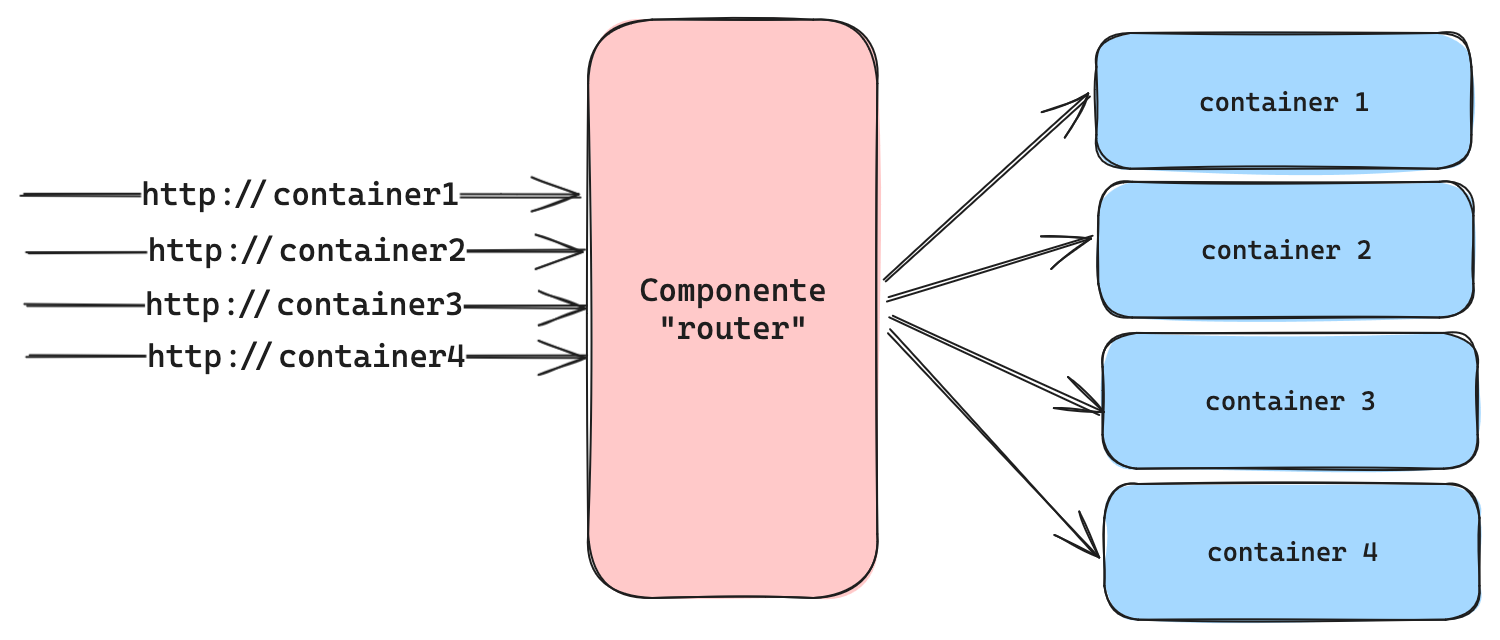
\includegraphics[width=1\textwidth]{files/images/routing-solution.png}
    \caption{Routing traffico verso container}
    \label{fig:routing}
\end{figure}
\newline
In questa maniera, l'unica porta esposta sull'host è quella sul componente "router", alla quale le richieste esterne potranno essere mandate, mentre sarà compito di quest'ultimo quello di instradare correttamente il traffico verso le porte interne, non esposte, dei vari container.
\subsubsection{Mancanza supporto per la gestione delle immagini Docker}
Allo stato attuale, la gestione delle immagini Docker per i vari notebook non è supportata. Uno dei requisiti dell'attività che ha portato a questa tesi è quello di creare un supporto al download e alla configurazione delle immagini che possono essere utilizzate per avviare i notebook, pertanto è stato sviluppato un componente \textit{ad-hoc} che verrà commentato successivamente.

\newpage
\section{NextPyter \textit{"2.0"}}
Analizzate le criticità del progetto nella versione \textit{"1.0"}, la sua architettura e le eventuali migliorie applicabili, il tema centrale di questa tesi sarà la descrizione del processo di progetto e sviluppo della versione \textit{"2.0"} della piattaforma, creata appositamente per apportare i cambiamenti richiesti, aggiungendo anche il supporto all'orchestratore di container \textit{Kubernetes}.
\newline
\begin{figure}[h]
    \centering
    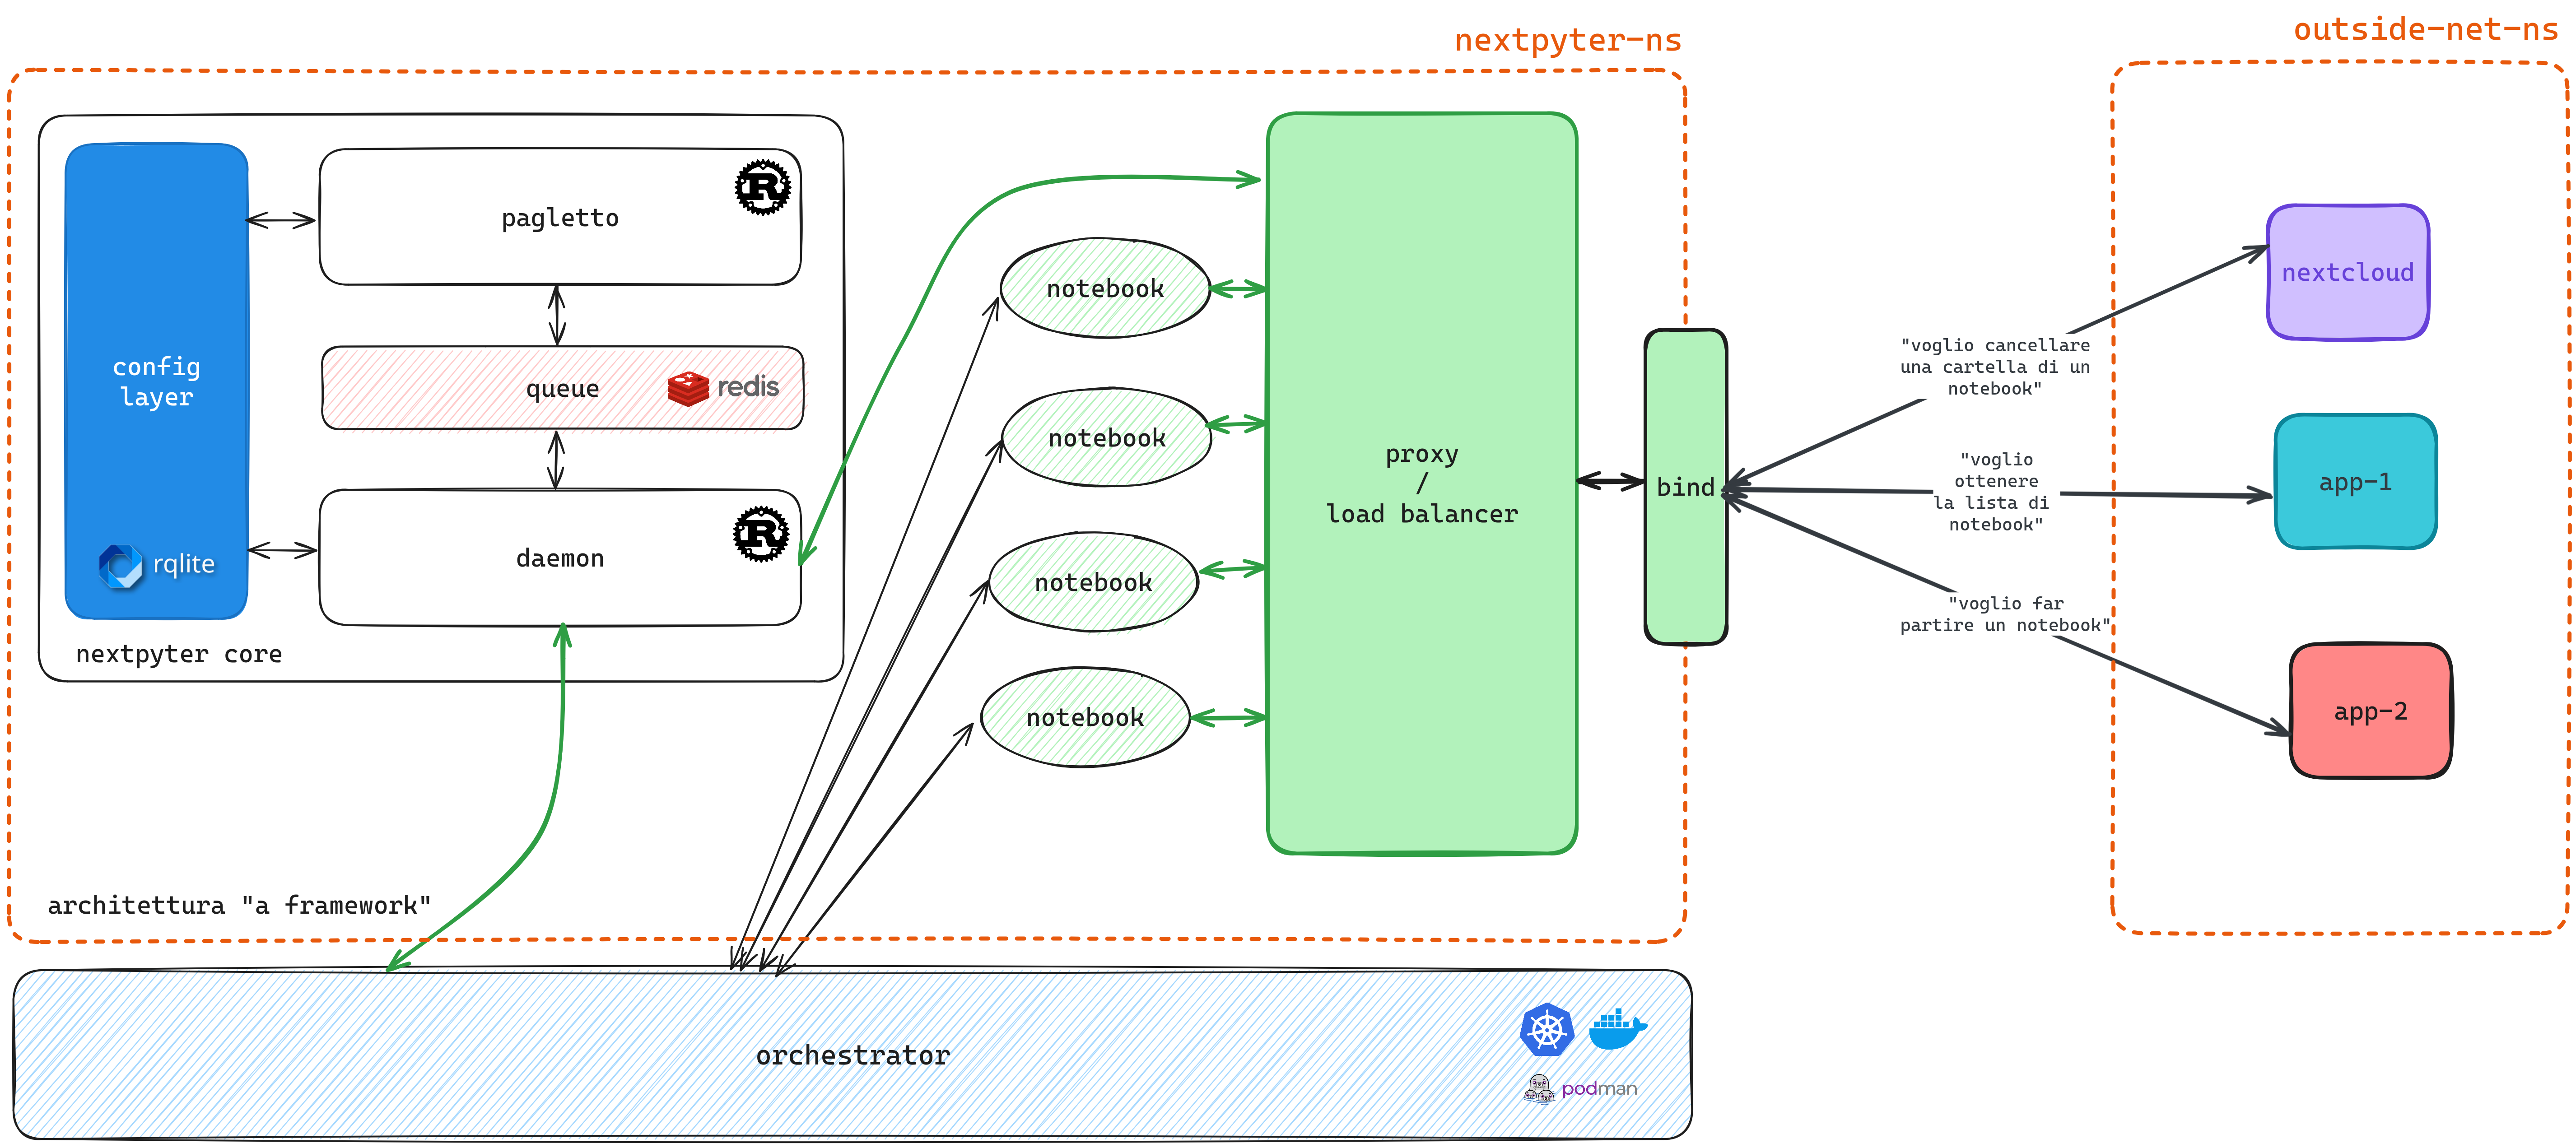
\includegraphics[width=1\textwidth]{files/images/nextpyter-2-diagram.png}
    \caption{Schema architetturale NextPyter \textit{"2.0"}}
    \label{fig:nextpyter-2-diagram}
\end{figure}
\newline
Sono stati identificati i seguenti nuovi obiettivi per NextPyter \textit{"2.0"}:
\begin{itemize}
    \item Supporto a Kubernetes: questo requisito non è stato esattamente identificato, semplicemente era il \textit{titolo dell'attività tirocinio}, pertanto è l'obiettivo "di arrivo" di questa tesi;
    \item Supporto alla \textit{high availability}: è stato individuato il bisogno di voler espandere la piattaforma ad una platea di utenti molto più grande. Da piattaforma installabile tramite Docker e Docker Compose, NextPyter dovrà trasformarsi in un'altra in grado di scalare orizzontalmente in modo da garantire il corretto soddisfacimento di più classi di traffico. Pertanto, non solo sarà necessario supportare Kubernetes, ma tutti i componenti che realizzano NextPyter, che analizzeremo successivamente, dovranno essere in grado di mostrare un determinato grado di \textit{resilienza}. In altre parole, NextPyter \textit{"2.0"} dovrà supportare egregiamente una quantità di traffico modellabile come le richieste provenienti da gruppi di ricerca di più dipartimenti dell'Università di Modena e Reggio Emilia, a grandi linee (eventualmente scalando oltre!);
    \item Miglioramento del supporto a Docker: nonostante la richiesta dell'implementazione del supporto a Kubernetes, è stato deciso di mantenere il supporto a Docker per supportare scenari più piccoli;
    \item Configurazione dinamica: allo stato attuale, la versione \textit{"1.0"} non prevede la configurazione dinamica delle immagini per i container dei notebook. La piattaforma \textit{"2.0"} dovrà essere in grado di supportare questo genere di requisito;
    \item Autorizzazione \textit{fine-grained} delle richieste: i componenti che vorranno interfacciarsi con NextPyter lo potranno fare mediante un set di permessi che verrà definito in un \textit{layer} di autenticazione che regolerà l'accesso al sistema in maniera estremamente granulare, usando un meccanismo che permetta di filtrare le richieste basandosi, virtualmente, su qualsiasi aspetto di quest'ultima;
\end{itemize}
\newline
In figura \ref{fig:nextpyter-2-diagram} è raffigurato un diagramma che illustra, ad alto livello, i nuovi componenti della piattaforma, che verranno approfonditi in dettaglio nei paragrafi a venire.
\newline
\subsection{NextPyter come \textit{framework}}
Una delle prime, se non la prima, necessità del progetto è stata sicuramente quella della creazione di un componente che scorporasse le funzionalità base di NextPyter da \textit{Nextcloud}: la complessità e profondità dei requisiti succitati non può fare affidamento su un componente del genere, perché troppo dipendente sulla presenza di un altro software. Le logiche che derivano, ad esempio, dal requisito riguardante la \textit{high availability} richiedono che ciascun componente del sistema scali indipendentemente rispetto agli altri, per riuscire a gestire volumi di traffico variabili: nella piattaforma \textit{"1.0"}, l'applicazione NextPyter non può scalare indipendentemente, poiché è strettamente vincolata all'ambiente in cui viene eseguita, ovvero \textit{Nextcloud} stesso.
\newline
L'idea fondamentale, quindi, è quella della realizzazione di un'entità a sé, con un perimetro ben definito all'interno del sistema: il cosiddetto \textit{core} di NextPyter.
\newline
La progettazione della nuova piattaforma ha visto la necessità di rendere le funzionalità base di NextPyter, la gestione di notebook Jupyter, quindi, un \textit{framework} accessibile tramite HTTP(S) dai più svariati client che vogliano implementarlo. In questo modo, NextPyter non è più legato necessariamente ad un'installazione di \textit{Nextcloud}, ma è estensibile da qualsiasi client voglia implementare le sue funzionalità, tramite interfacce che verranno descritte in maggior dettaglio fra qualche paragrafo.
\subsubsection{Controllo dei container: il modulo \textit{daemon}}
Il modulo di "rappresentanza" del \textit{core} di NextPyter è sicuramente il \textit{daemon}, poiché esporrà l'API HTTP che permetterà di poter interagire con le logiche di NextPyter.
\newline
Questo modulo dovrà essere realizzato tenendo a mente i seguenti principi:
\begin{itemize}
    \item Riduzione della \textit{attack surface} derivante dall'approccio \textit{DinD}: dal momento in cui NextPyter dovrà comunque supportare Docker, è stato necessario revisionare l'approccio all'interazione col \textit{Docker daemon}. In particolare, l'unico componente che avrà accesso al socket di Docker sarà il \textit{daemon} di NextPyter e tutti gli altri componenti del sistema, ogniqualvolta vorranno fare operazioni riguardanti la gestione dei notebook, dovranno riferirsi al \textit{daemon} stesso. L'approccio è il medesimo descritto nel paragrafo \ref{dind-acceptable};
    \item Least privilege: i client che vorranno interfacciarsi a \textit{daemon} lo faranno utilizzando un set di richieste specifiche che verranno filtrate appositamente dal layer di autenticazione e autorizzazione descritto in precedenza. In questo modo, tramite un set di regole ben definite, client diversi potranno accedere in maniere diverse e completamente personalizzabili al sistema;
    \item Isolamento delle risorse: come già ancitipato, qualsiasi componente del \textit{core} dovrà essere in grado di scalare orizzontalmente (e verticalmente, volendo);
    \item Minimizzazione delle dipendenze: NextPyter deve essere progettato in modo da ridurre non solo le dipendenze di traffico, ma anche quelle di codice. A questo pro, per l'appunto, è stata sviluppata l'interfaccia HTTP di cui sopra, per realizzare un protocollo implementabile da qualsiasi client;
    \item Astrazione dell'orchestratore di \textit{container}: poiché la piattaforma dovrà supportare sia Docker che Kubernetes, sarà necessario sviluppare l'API REST in una maniera che prescinde completamente dal tipo di orchestratore con la quale il modulo andrà a comunicare. I client che si interfacceranno con \textit{daemon} non avranno la necessità di sapere se quest'ultimo sia in collegamento con Kubernetes o con Docker: tutto sarà completamente trasparente agli utilizzatori e l'interfaccia sarà la medesima in entrambi i casi, semplificando nettamente lo sviluppo dei client.
\end{itemize}
\subsubsection{Configurazione dinamica: il modulo \textit{pagletto}, \textit{RQLite} e \textit{Valkey}}
Questo modulo, dal nome che non significa particolarmente nulla, accoppiato ad un database ad alta disponibilità, \textit{RQLite} e \textit{Valkey}, un database \textit{key-value}, soddisferà il requisito di configurazione dinamica delle immagini. In particolare, come visibile anche dallo schema, sarà possibile, mediante una chiamata API HTTP fatta verso \textit{daemon}, richiedere il download di un'immagine \textit{Docker} dal \textit{registry} ufficiale (configurabile, eventualmente). Questa immagine, una volta scaricata, verrà registrata nel database \textit{RQLite}\footnote{https://rqlite.io/}, un \textit{fork} di \textit{SQLite} progettato per essere leggero e \textit{highly available}.\newline
Infatti, RQLite è un database SQL che è in grado di replicare i dati per questioni di \textit{fault tolerance}, rendendoli disponibili tra più nodi, in modo che se uno di questi è soggetto a malfunzionamenti, l'accesso sia comunque garantito dai rimanenti. Oltre a questo, RQLite funziona mediante un protocollo a elezione di \textit{leader}, \textbf{\textit{raft}}\footnote{https://raft.github.io/}, pertanto vi saranno copie autoritative e copie non autoritative dei dati, in modo da garantire che lo stato del database sia sempre integro. Questo tipo di database è stato scelto perché è implementato in maniera estremamente semplice, astraendo tutte le chiamate di basso livello attraverso, anche qui, una API REST.
A questo punto, gli unici container avviabili, sempre tramite un'apposita chiamata HTTP, saranno quelli che avranno immagini che compaiono all'interno della configurazione distribuita, rendendo più sicura l'interazione con l'orchestratore da parte di \textit{daemon}.
\newline
Per realizzare la comunicazione tra \textit{daemon} e \textit{pagletto} sarà utilizzato \textit{Valkey}, un database \textit{key-value}, il \textit{fork open source} del progetto \textit{Redis}\footnote{https://www.linuxfoundation.org/press/linux-foundation-launches-open-source-valkey-community}, sfruttando la tecnologia di \textit{event streaming} fornita da Valkey stesso, che verrà dettagliata nei prossimi paragrafi. 

\subsubsection{Utilizzo di NGINX per ottimizzare la gestione delle risorse di rete: il modulo \textit{proxy}}
Come già anticipato in sezione \ref{net-acceptable}, la versione \textit{"1.0"} di NextPyter gestiva le risorse di rete in maniera subottimale. Per sopperire a questo problema, è stato deciso di implementare il \textit{routing} del traffico di tutto il \textit{core} mediante l'utilizzo di \textit{NGINX} configurato come \textit{reverse proxy}.
\newline
Un reverse proxy è un componente di rete che si interpone tra la comunicazione fra client e server, in questo caso i \textit{notebook}, principalmente, con lo scopo di gestire e regolare le richieste in entrata al sistema, eventualmente modificandole o validandole mediante un qualche genere di logica (anche personalizzata).
\newline
NGINX, nell'ecosistema NextPyter, viene usato proprio a questo scopo: viene interposto fra la comunicazione con l'esterno e i notebook, in modo da fornire una serie di garanzie che senza di esso sarebbe difficile fornire, come ad esempio la verifica dell'autenticità delle richieste, il bilanciamento delle richieste in arrivo e, tra le altre cose, il "mascheramento" delle porte dei notebook verso l'esterno. La configurazione di NGINX, infatti, è sostanzialmente la stessa che viene proposta nella sezione \ref{net-acceptable}, che verrà dettagliata maggiormente nel prossimo capitolo, dove verrà descritta l'implementazione dell'architettura di NextPyter \textit{"2.0"}.
\newline
Oltre a questo, NGINX verrà utilizzato per via della sua ampia estensibilità: infatti, oltre ad essere un \textit{load balancer}, NGINX è configurabile per essere \textit{application gateway}, ovvero un componente che è in grado di trascendere dal classico ruolo di bilanciatore del traffico e implementare l'indirizzamento delle richieste basandosi su logiche completamente personalizzate.
\newline
Questo obiettivo verrà realizzato mediante \textit{NJS}, sostanzialmente un motore JavaScript progettato per l'utilizzo all'interno di NGINX. Creato per estendere le capacità di scripting del server NGINX, \textit{NJS} consente di manipolare le richieste HTTP e le risposte in tempo reale, facilitando la gestione avanzata delle richieste, la modifica delle intestazioni, il controllo degli accessi, il routing dinamico e altre personalizzazioni senza compromettere le prestazioni. Questo linguaggio è integrato direttamente in NGINX, consentendo l'esecuzione di script lato server in modo efficiente e sicuro, con un impatto minimo sulle prestazioni del server web.
\subsubsection{Documentazione autogenerate: il modulo \textit{docs}}
Per via della natura dell'ecosistema di NextPyter \textit{"2.0"}, è stato ritenuto opportuno includere un modulo che permettesse la consultazione della documentazione dell'API HTTP fornita dal modulo \textit{daemon} in maniera semplice e \textit{user-friendly}.
\newline
A questo scopo, sfruttando lo standard OpenAPI, verrà messo a punto un sistema per il quale, una volta che \textit{daemon} verrà compilato, sarà creato un \textit{endpoint} HTTP che espone la documentazione riguardante la API REST seguendo lo standard \textit{openapi 3.0}. Una volta esposto l'endpoint, verrà messo a punto un altro modulo, \textit{docs}, che interperllerà tale endpoint di documentazione, effettuerà operazioni di \textit{parsing} e lo presenterà tramite un'interfaccia \textit{user friendly}. Questo modulo sarà reso disponibile utilizzando \textit{Swagger UI}\footnote{https://swagger.io/tools/swagger-ui/}, uno strumento open-source utilizzato per visualizzare e interagire con le API web che seguono la specifica OpenAPI (precedentemente nota come Swagger Specification). È un'interfaccia grafica che consente alle sviluppatrici e agli sviluppatori di esplorare, testare e documentare le API in modo interattivo.
\begin{figure}[h]
    \centering
    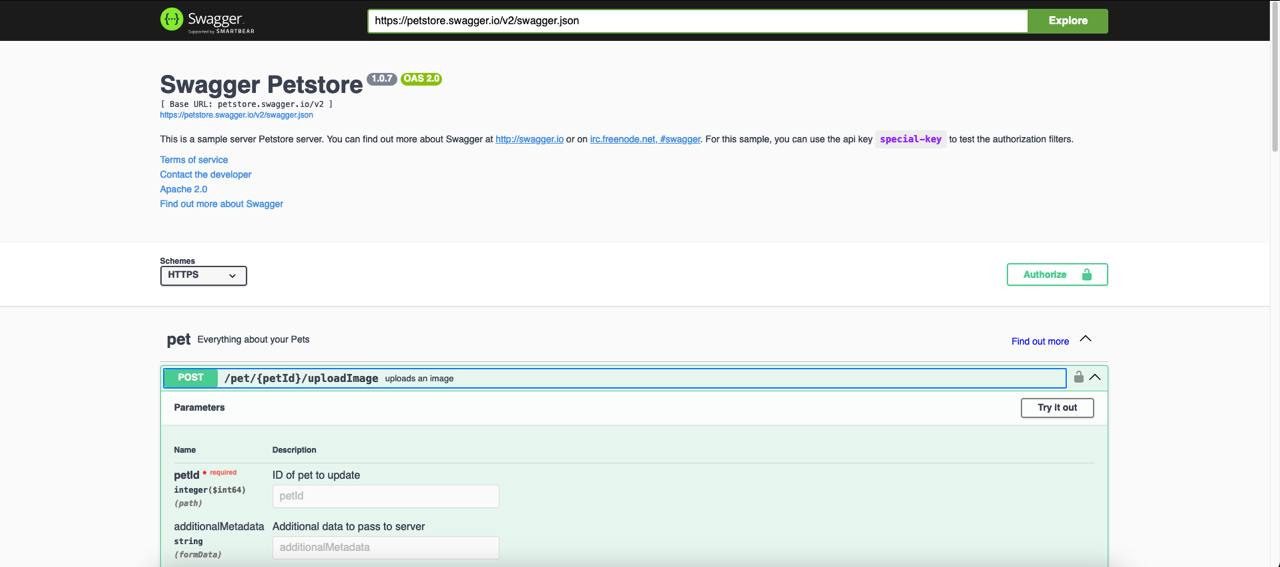
\includegraphics[width=1\textwidth]{files/images/swagger-ui.jpg}
    \caption{Interfaccia di Swagger UI}
    \label{fig:swagger-ui}
\end{figure}

\subsubsection{Sommario}
Nella progettazione di NextPyter \textit{"2.0"}, è stata posta particolare enfasi sulla modularità e l'indipendenza del sistema, elementi chiave per superare le limitazioni della versione 1.0. In quest'ultima, la piattaforma era strettamente vincolata a Nextcloud, il che limitava fortemente la capacità di scalare e adattarsi alle nuove esigenze. La nuova architettura si distacca radicalmente da questo modello, adottando un approccio modulare che separa chiaramente le varie funzionalità del sistema. Questo consente di gestire, aggiornare e migliorare ciascun componente in modo indipendente, riducendo le interdipendenze che complicano la manutenzione e l'evoluzione della piattaforma. Ciò permette al sistema di scalare orizzontalmente, gestendo efficacemente grandi volumi di traffico e garantendo alta disponibilità e resilienza, elementi fondamentali per supportare le richieste di gruppi di ricerca diversi e numerosi. Inoltre, l'indipendenza dei moduli consente alla piattaforma di evolversi più facilmente, integrando nuove tecnologie o migliorando quelle esistenti senza necessità di ristrutturazioni complesse o invasive. Questa flessibilità rappresenta un notevole passo avanti rispetto alla versione precedente, rendendo NextPyter 2.0 una piattaforma più robusta, adattabile e pronta per future sfide e opportunità di espansione.

\subsection{Progettazione layer di autenticazione}
Per mantenere le faccende quanto più modulari e indipendenti possibili, è stato scelto di rendere il \textit{layer} di autenticazione, almeno in questa fase iniziale della nuova piattaforma, un componente facoltativo, sottolineando un'altra volta la estrema modularità del sistema.
\newline
Nell'immagine \ref{fig:nextpyter-2-diagram}, si può notare come questo modulo sia presente, quando attivato, in tutte le interazioni che vengono fatte all'interno del sistema, per garantire, appunto, sicurezza e autenticità nelle transazioni.
\newline
Il tipo protocollo che si è deciso di supportare è \textit{OAuth2}, sostanzialmente lo standard \textit{de-facto} \cite{auth0} dell'industria per quanto riguarda autenticazione e autorizzazione tra microservizi.
\newline
\subsubsection{Cos'è OAuth2}
\textit{Premessa: questa sezione è stata tratta, tradotta e adattata da un progetto dell'autore della tesi \footnote{https://github.com/emilianomaccaferri/oauth2-spring-boot/blob/main/chapters/Chapter\%20I.md}}.
\newline
\newline
OAuth2 è uno \textit{standard}, un \textit{protocollo}, come già menzionato, non qualcosa che è possibile "eseguire", che permette di definire un set di operazioni che realizzano l'autenticazione e l'autorizzazione in un determinato sistema.\newline
Per poter utilizzare questo standard, dunque, è necessario utilizzare un cosiddetto \textit{identity provider}, o \textit{IDP}, che implementi \textit{OAuth2}, sostanzialmente un software che realizza ciò che viene definito nello standard.
\newline
Uno degli IDP di più rilievo è sicuramente Keycloak \cite{keycloak-stats}, sviluppato e mantenuto da \textit{RedHat}. Oltre a questo, Keycloak è completamente open source e utilizzabile come software \textit{self-hosted}, rendendolo la scelta perfetta per un sistema con i vincoli, anche di dipendenza da \textit{vendor} di servizi cloud, di NextPyter.

\subsubsection{OAuth2 in dettaglio}
Come si ottiene accesso ad un set di risorse protette da un IDP OAuth2? La risposta è semplice, mediante l'utilizzo di un \textbf{flow}, un insieme di "passi" che l'IDP metterà in atto per verificare l'identità di un client che vuole accedere al sistema.
\newline
I principali flow che verranno descritti in questa sezione sono l'\textit{authorization code flow} e il \textit{service account flow} (nota: i nomi di questi flow possono cambiare da IDP a IDP, in questa sezione sono stati usati i nomi più utilizzati nell'industria). 
\newline
Il primo è utilizzato quando il client che sta cercando di accedere alle risorse protette è un sito web o un'applicazione mobile, o comunque qualsiasi tipo di applicazione la cui interazione con il sistema è guidata da un utente, mentre il secondo tipo di flow viene utilizzato da applicazioni che non sono guidate da utenti, come servizi di automazione, servizi di logging, script esterni, microservizi e quant'altro.
\newline
Entrambi i flow, comunque, utilizzano due informazioni molto importanti, cruciali nella realizzazione di tutte logiche di autenticazione e autorizzazione: \textit{access token} e \textit{refresh token}.
\begin{itemize}
    \item Un \textit{access token} viene utilizzato per effettuare \textbf{richieste autenticate} al sistema. La caratteristica principale di questo tipo di token è che hanno una vita particolarmente breve, per via del fatto che questo genere di informazioni, ovvero quelle che permettono l'accesso diretto ad un sistema, sono soggette a \textbf{leak}, i protocolli di sicurezza vengono \textbf{penetrati}, insomma, tante cose possono andare male, pertanto ha senso \textit{agire in favore di sicurezza} e dare un \textit{TTL} basso a questo genere di token;
    \item Un \textit{refresh token}, invece, viene utilizzato per \textbf{ottenere nuovi \textit{access token}} quando questi scadono. Questi, a differenza degli altri, hanno un \textit{TTL} particolarmente lungo e, per questo motivo, vanno mantenuti con particolare scrupolo.
\end{itemize}
\newpage
\subsubsection{Funzionamento dell'\textit{authorization code flow}}
Per descrivere in maniera concisa il funzionamento di questo processo, verrà utilizzata come riferimento l'immagine \ref{fig:auth-code-flow} qui sotto.
\begin{figure}[h]
    \centering
    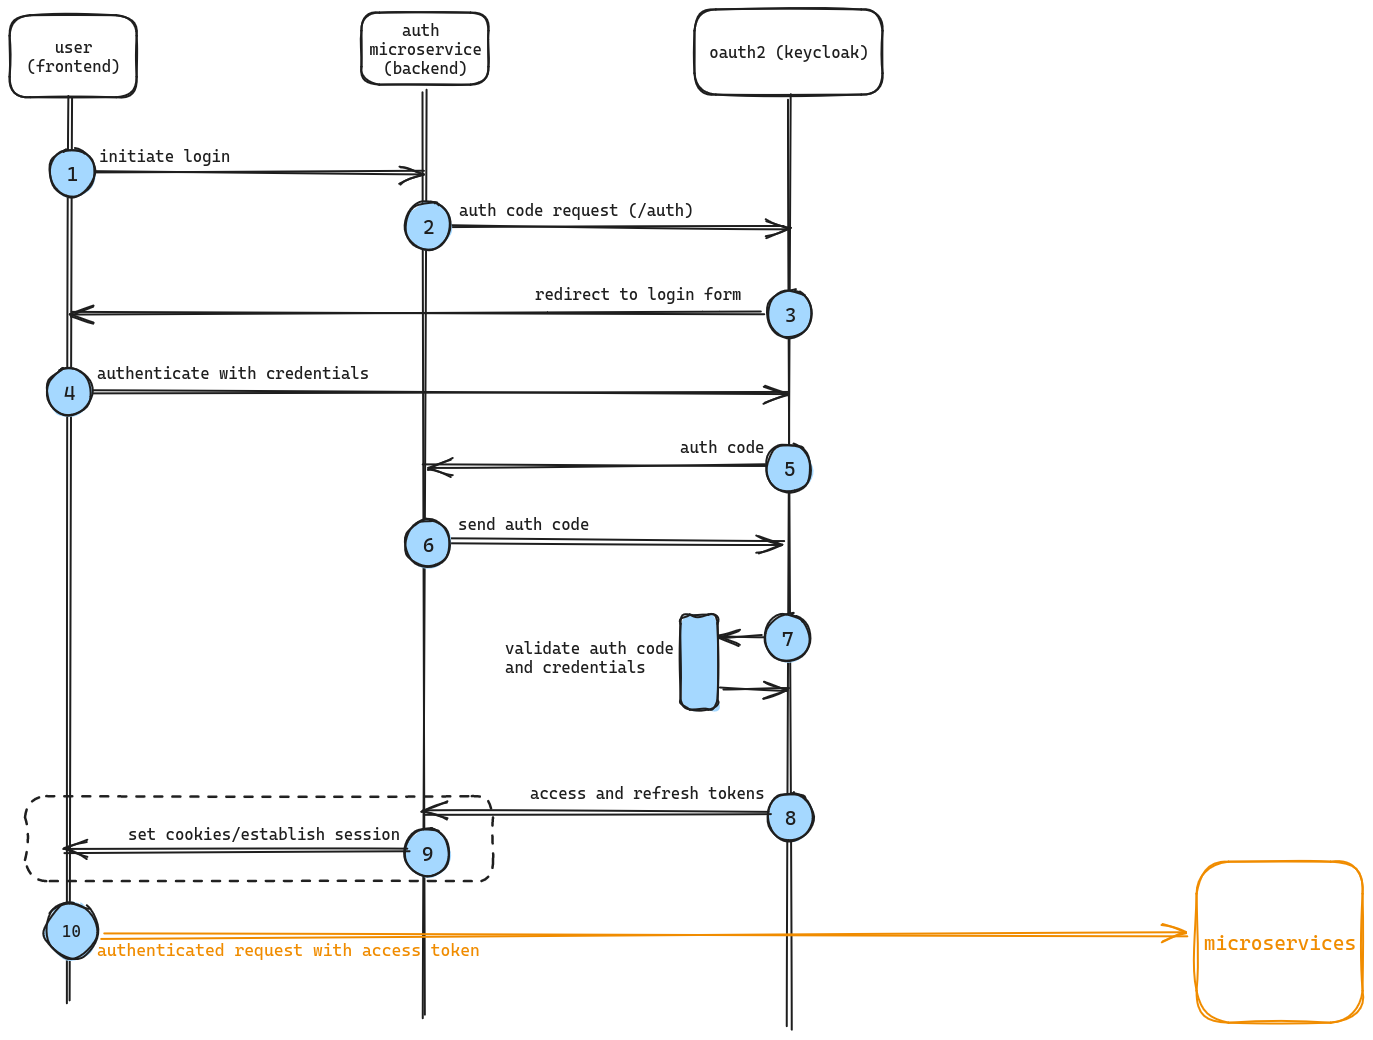
\includegraphics[width=1\textwidth]{files/images/auth-code-flow.png}
    \caption{Authorization code flow}
    \label{fig:auth-code-flow}
\end{figure}
\newline
Il flusso può essere dettagliato come segue:
\begin{itemize}
    \item L'utente clicca sul classico bottone di login;
    \item Il backend del sito web su cui viene effettuata la richiesta di login effettua una cosiddetta \textit{authorization code request}. Questa azione fa ridirigere l'utente al form di login (che può essere il classico \textit{"Login con Google"} o equivalenti);
    \item L'utente viene ridiretto al form di login;
    \item L'utente si autentica;
    \item Se le credenziali sono corrette, un \textit{auth code} è inviato al backend iniziale, quello del sito d'origine;
    \item Una volta che l'\textit{auth code} è stato ricevuto dal backend, questo effettua un'ulteriore richiesta per ottenere gli \textit{access} e \textit{refresh token}. Notare come la presenza di un \textit{auth code} sia critica per mitigare una serie di rischi di sicurezza non banali: emettendo un \textit{auth code}, il client di origine \textbf{non contatta mai direttamente l'\textit{IDP}} che regola l'accesso al sistema e il processo di autenticazione è completamente delegato a \textit{backend} e \textit{IDP}. Questa cosa rafforza particolarmente la sicurezza del processo e, in particolare, non permette accesso privilegiato \textbf{diretto} all'\textit{IDP} da parte di client potenzialmente vulnerabili. Se, ad esempio, il token non venisse passato direttamente al server, ma venisse passato ad un client vulnerabile, l'\textit{auth code} sarebbe rubato e l'intero flusso di autenticazione sarebbe corrotto, permettendo ad attaccanti esterni di autenticarsi come se fossero il client legittimo! Quello che accade, invece, è che il backend richiede le credenziali (i token di cui sopra) con l'\textit{auth code} e l'\textit{IDP} è configurato per ricevere richieste di autenticazione solo da tale servizio, rafforzando ancora di più la sicurezza del processo;
    \item L'IDP verifica le credenziali e l'\textit{auth code} presentato;
    \item I token vengono emessi e...
    \item ... una sessione di autenticazione viene creata tra frontend e backend;
    \item L'utente potrà fare, ora, richieste autenticate al sistema.
\end{itemize}
\newpage
\subsubsection{Funzionamento \textit{service account flow}}
Come già menzionato, i \textit{service account} sono tutte quelle applicazioni "autonome" e non guidate da utenti, come aggregatori di log, servizi di notifiche, ...\newline
In maniera del tutto analoga al caso precedente, verrà utilizzata l'immagine \ref{fig:sa-flow} per descrivere il funzionamento del \textit{service account flow}.
\begin{figure}[h]
    \centering
    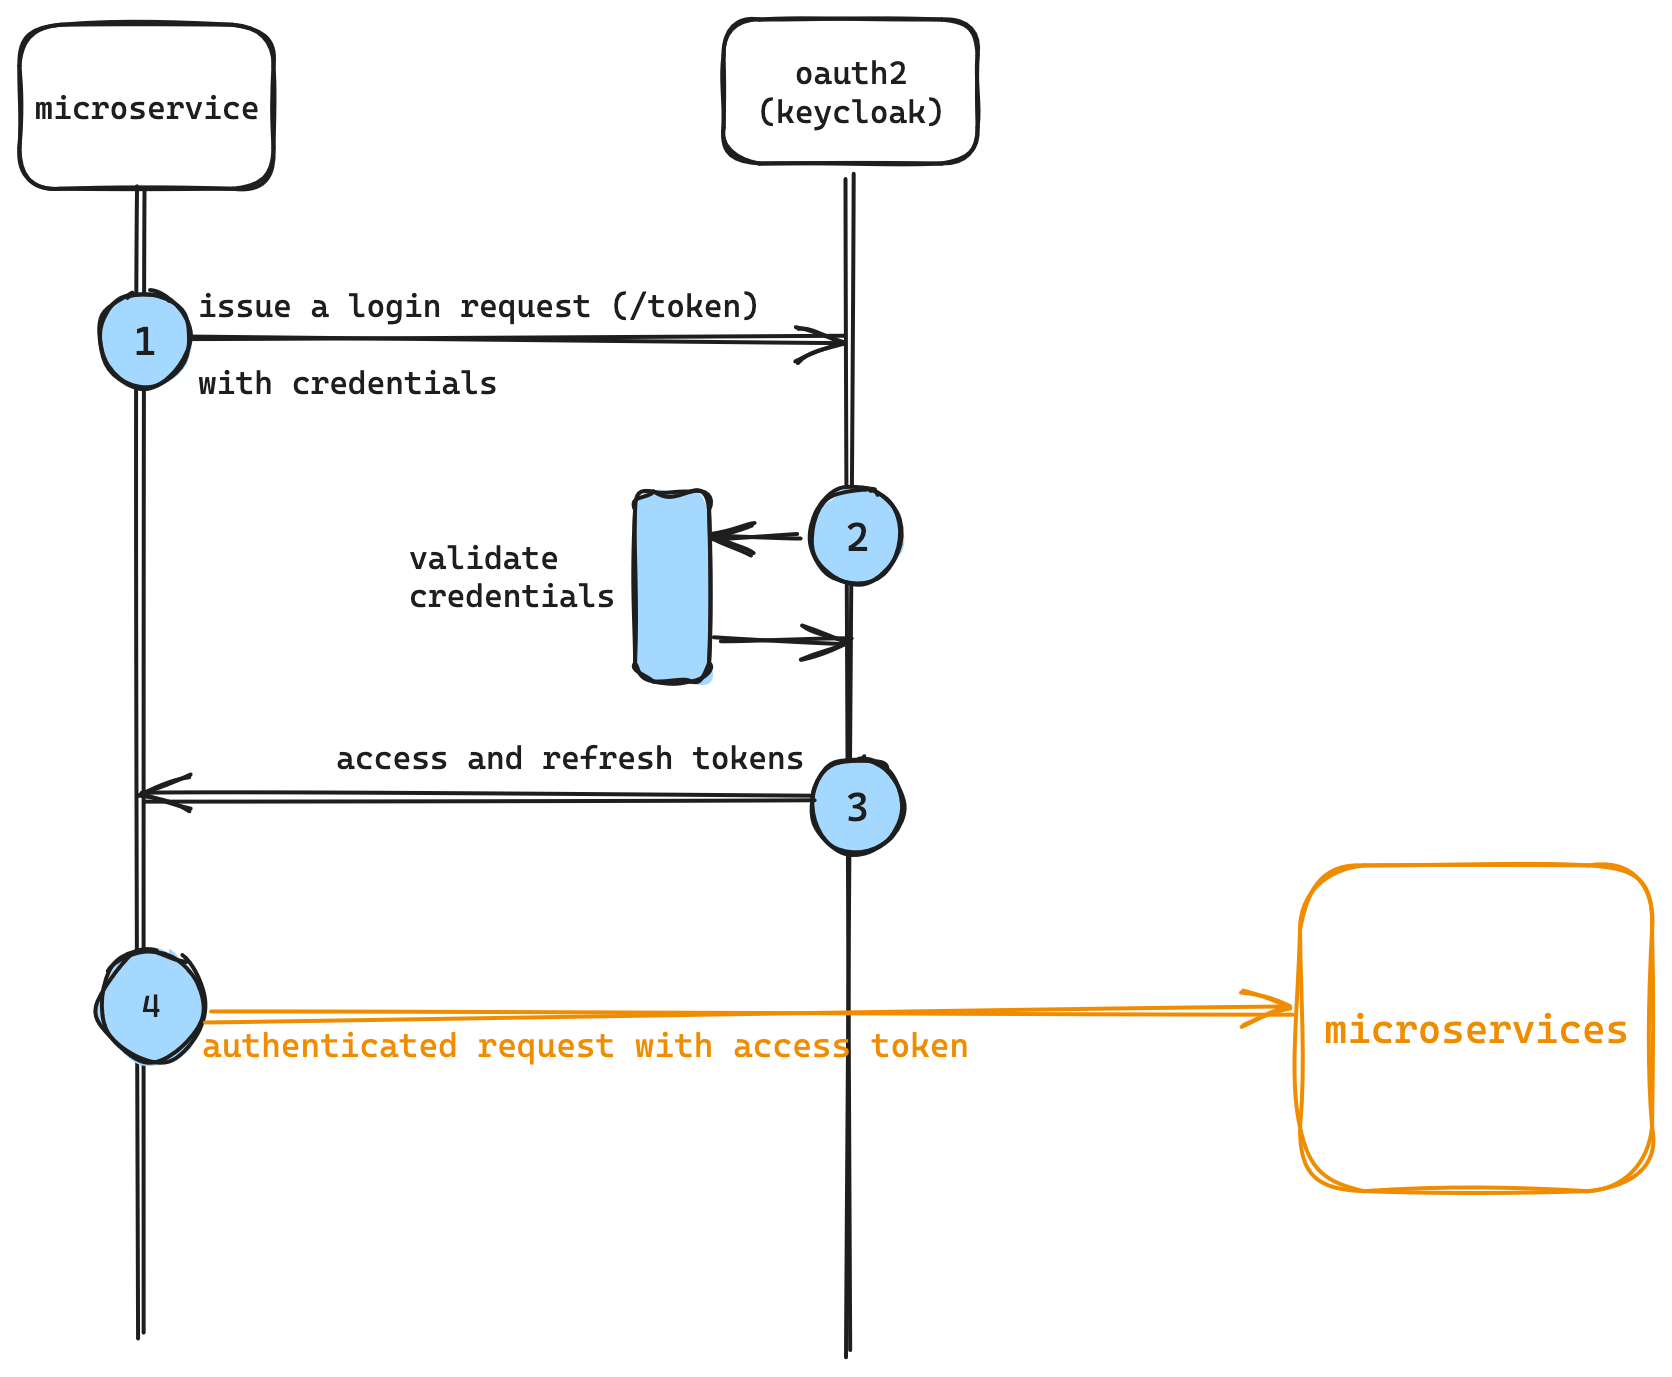
\includegraphics[width=1\textwidth]{files/images/service-account-flow.png}
    \caption{Service account flow}
    \label{fig:sa-flow}
\end{figure}
Come si può ben vedere, questo flusso è molto più semplice del precedente:
\begin{itemize}
    \item Il servizio ha delle credenziali pre-generate con le quali effettuare la richiesta per dei token;
    \item L'IDP valida le credenziali...
    \item ...e ritorna i token al servizio;
    \item In questo modo, il servizio in questione potrà effettuare richieste autenticate senza dover specificare sempre le proprie credenziali (come, ad esempio, succede con la \textit{Basic Auth}), riducendo la probabilità che queste vengano intercettate da agenti malevoli.
\end{itemize}

Per più dettagli sul funzionamento di questo protocollo e sulle attività ad esso riguardanti, è consigliabile consultare questo progetto\footnote{https://github.com/emilianomaccaferri/oauth2-spring-boot/tree/main}, di opera dell'autore di questa tesi.

\subsubsection{Keycloak}
Keycloak è una soluzione open-source di Identity and Access Management (IAM) sviluppata da Red Hat, progettata per semplificare l'autenticazione e l'autorizzazione nelle applicazioni moderne. Supporta protocolli standard come OpenID Connect, OAuth 2.0 e SAML 2.0, rendendolo compatibile con una vasta gamma di applicazioni e servizi. Keycloak consente di gestire centralmente utenti, ruoli, permessi e sessioni, offrendo funzionalità di Single Sign-On (SSO), federazione di identità, autenticazione a più fattori (MFA) e controllo di accesso basato su ruoli (RBAC). La sua architettura flessibile permette l'integrazione con directory LDAP, Active Directory, database relazionali e provider di identità esterni. Inoltre, Keycloak fornisce un'interfaccia utente web intuitiva per la gestione delle identità e offre API REST per l'integrazione programmatica.
\newline
Per via della sua estrema flessibilità e personalizzabilità, è stato scelto come \textit{IDP} per il progetto NextPyter.
\begin{figure}[h]
    \centering
    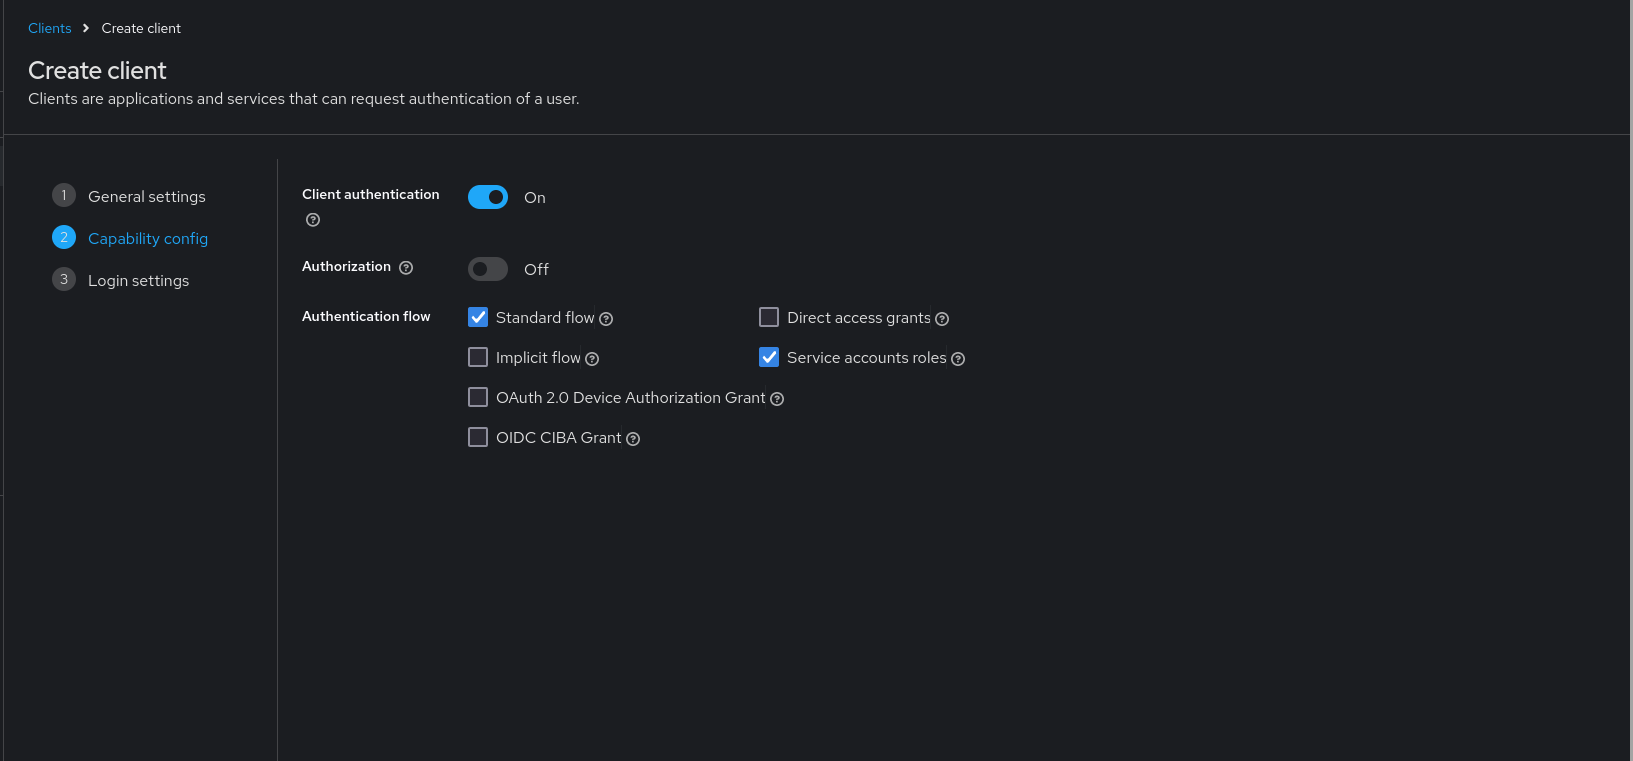
\includegraphics[width=1\textwidth]{files/images/keycloak.png}
    \caption{Una lista di flow supportati da Keycloak}
    \label{fig:keycloak-clients}
\end{figure}
\newline
In particolare, è possibile configurare Nextcloud in maniera tale che utilizzi un'istanza di Keycloak come provider di autenticazione e, di conseguenza, controllare le richieste e i permessi degli utenti dall'\textit{application gateway} citato in precedenza, poiché le credenziali che verranno emesse agli utenti di Keycloak saranno sotto forma di JWT, un formato di dati ispezionabile e crittograficamente verificabile.